\subsection{IASI Band 2 (1210-2000\invcm)}
%-----------------------------------------

\subsubsection{WVO-derived residuals}
%....................................
IASI band 2 brightness temperature residuals for all the WVO1 set of transmittances are shown in figure \ref{fig:iasiB2.wvo1_dtb_sfc}, with the average, RMS, and maximum residuals shown in figure \ref{fig:iasiB2.wvo1_dtb}. Figures \ref{fig:iasiB2.wvo2_dtb_sfc} and \ref{fig:iasiB2.wvo2_dtb} show the same for the WVO2 set of transmittances.

Both the WVO1 and WVO2 results are similar with the most visible difference in the spectral region 1700-1850\invcm{} where the WVO1 residuals are a tiny bit noisier.
\begin{figure}[htp]
  \centering
  \includegraphics[scale=0.8]{graphics/iasiB2/iasiB2.wvo1_dtb_sfc.eps}
  \caption{IASI band 2 brightness temperature residuals for all view angles and profiles between using the true total transmittance profiles and those derived from the WVO1 set (see table \ref{tab:derived_set_combo})}
  \label{fig:iasiB2.wvo1_dtb_sfc}
  \vspace{1em}
  \includegraphics[scale=0.8]{graphics/iasiB2/iasiB2.wvo1_dtb.eps}
  \caption{IASI band 2 brightness temperature residual statistics between using the true total transmittance profiles and those derived from the WVO1 set (see table \ref{tab:derived_set_combo}). Compiled for all view angle and profile combinations. \textbf{(Top panel)} Average T\subscript{B} residuals. \textbf{(Middle panel)} RMS T\subscript{B} residuals. \textbf{(Bottom panel)} Maximum T\subscript{B} residuals.}
  \label{fig:iasiB2.wvo1_dtb}
\end{figure}
\begin{figure}[htp]
  \centering
  \includegraphics[scale=0.8]{graphics/iasiB2/iasiB2.wvo2_dtb_sfc.eps}
  \caption{IASI band 2 brightness temperature residuals for all view angles and profiles between using the true total transmittance profiles and those derived from the WVO2 set (see table \ref{tab:derived_set_combo})}
  \label{fig:iasiB2.wvo2_dtb_sfc}
  \vspace{1em}
  \includegraphics[scale=0.8]{graphics/iasiB2/iasiB2.wvo2_dtb.eps}
  \caption{IASI band 2 brightness temperature residual statistics between using the true total transmittance profiles and those derived from the WVO2 set (see table \ref{tab:derived_set_combo}). Compiled for all view angle and profile combinations. \textbf{(Top panel)} Average T\subscript{B} residuals. \textbf{(Middle panel)} RMS T\subscript{B} residuals. \textbf{(Bottom panel)} Maximum T\subscript{B} residuals.}
  \label{fig:iasiB2.wvo2_dtb}
\end{figure}


\subsubsection{DOZ-derived residuals}
%....................................
IASI band 2 brightness temperature residuals for all the DOZ1 set of transmittances are shown in figure \ref{fig:iasiB2.doz1_dtb_sfc}, with the average, RMS, and maximum residuals shown in figure \ref{fig:iasiB2.doz1_dtb}. Figures \ref{fig:iasiB2.doz2_dtb_sfc} and \ref{fig:iasiB2.doz2_dtb} show the same for the DOZ2 set of transmittances.

As with the WVO results, both the DOZ1 and DOZ2 results are similar. However, the magnitude of the statistics for these transmittances are nearly two orders of magnitude \emph{less} than for the WVO results across the entire band.
\begin{figure}[htp]
  \centering
  \includegraphics[scale=0.8]{graphics/iasiB2/iasiB2.doz1_dtb_sfc.eps}
  \caption{IASI band 2 brightness temperature residuals for all view angles and profiles between using the true total transmittance profiles and those derived from the DOZ1 set (see table \ref{tab:derived_set_combo})}
  \label{fig:iasiB2.doz1_dtb_sfc}
  \vspace{1em}
  \includegraphics[scale=0.8]{graphics/iasiB2/iasiB2.doz1_dtb.eps}
  \caption{IASI band 2 brightness temperature residual statistics between using the true total transmittance profiles and those derived from the DOZ1 set (see table \ref{tab:derived_set_combo}). Compiled for all view angle and profile combinations. \textbf{(Top panel)} Average T\subscript{B} residuals. \textbf{(Middle panel)} RMS T\subscript{B} residuals. \textbf{(Bottom panel)} Maximum T\subscript{B} residuals.}
  \label{fig:iasiB2.doz1_dtb}
\end{figure}
\begin{figure}[htp]
  \centering
  \includegraphics[scale=0.8]{graphics/iasiB2/iasiB2.doz2_dtb_sfc.eps}
  \caption{IASI band 2 brightness temperature residuals for all view angles and profiles between using the true total transmittance profiles and those derived from the DOZ2 set (see table \ref{tab:derived_set_combo})}
  \label{fig:iasiB2.doz2_dtb_sfc}
  \vspace{1em}
  \includegraphics[scale=0.8]{graphics/iasiB2/iasiB2.doz2_dtb.eps}
  \caption{IASI band 2 brightness temperature residual statistics between using the true total transmittance profiles and those derived from the DOZ2 set (see table \ref{tab:derived_set_combo}). Compiled for all view angle and profile combinations. \textbf{(Top panel)} Average T\subscript{B} residuals. \textbf{(Middle panel)} RMS T\subscript{B} residuals. \textbf{(Bottom panel)} Maximum T\subscript{B} residuals.}
  \label{fig:iasiB2.doz2_dtb}
\end{figure}


\subsubsection{WVD-derived residuals}
%....................................
IASI band 2 brightness temperature residuals for all the WVD1 set of transmittances are shown in figure \ref{fig:iasiB2.wvd1_dtb_sfc}, with the average, RMS, and maximum residuals shown in figure \ref{fig:iasiB2.wvd1_dtb}. Figures \ref{fig:iasiB2.wvd2_dtb_sfc} and \ref{fig:iasiB2.wvd2_dtb} show the same for the WVD2 set of transmittances.

Unlike the WVO and DOZ residuals, the WVD results are different between the WVD1 and WVD2 sets. The WVD1 residuals are almost identical to those for WVO1 (see either figure \ref{fig:iasiB2.wvo1_dtb} or \ref{fig:iasiB2.wvo2_dtb}), whereas the WVD2 residuals do not have the individual frequency peaks (e.g. such as at 1363.25 and 1908.0\invcm{}) seen in the WVO results so the previosuly mentioned ``noisy'' region around 1675-1900\invcm{} seen in the WVO1 results is emphasised.
\begin{figure}[htp]
  \centering
  \includegraphics[scale=0.8]{graphics/iasiB2/iasiB2.wvd1_dtb_sfc.eps}
  \caption{IASI band 2 brightness temperature residuals for all view angles and profiles between using the true total transmittance profiles and those derived from the WVD1 set (see table \ref{tab:derived_set_combo})}
  \label{fig:iasiB2.wvd1_dtb_sfc}
  \vspace{1em}
  \includegraphics[scale=0.8]{graphics/iasiB2/iasiB2.wvd1_dtb.eps}
  \caption{IASI band 2 brightness temperature residual statistics between using the true total transmittance profiles and those derived from the WVD1 set (see table \ref{tab:derived_set_combo}). Compiled for all view angle and profile combinations. \textbf{(Top panel)} Average T\subscript{B} residuals. \textbf{(Middle panel)} RMS T\subscript{B} residuals. \textbf{(Bottom panel)} Maximum T\subscript{B} residuals.}
  \label{fig:iasiB2.wvd1_dtb}
\end{figure}
\begin{figure}[htp]
  \centering
  \includegraphics[scale=0.8]{graphics/iasiB2/iasiB2.wvd2_dtb_sfc.eps}
  \caption{IASI band 2 brightness temperature residuals for all view angles and profiles between using the true total transmittance profiles and those derived from the WVD2 set (see table \ref{tab:derived_set_combo})}
  \label{fig:iasiB2.wvd2_dtb_sfc}
  \vspace{1em}
  \includegraphics[scale=0.8]{graphics/iasiB2/iasiB2.wvd2_dtb.eps}
  \caption{IASI band 2 brightness temperature residual statistics between using the true total transmittance profiles and those derived from the WVD2 set (see table \ref{tab:derived_set_combo}). Compiled for all view angle and profile combinations. \textbf{(Top panel)} Average T\subscript{B} residuals. \textbf{(Middle panel)} RMS T\subscript{B} residuals. \textbf{(Bottom panel)} Maximum T\subscript{B} residuals.}
  \label{fig:iasiB2.wvd2_dtb}
\end{figure}
